\documentclass[16.7pt]{jsarticle}

\usepackage{SPR}

\headerSPR
\begin{document}
	\titleSPR{\number\year}{\number\month}{\number\day}{D2}{吉田 皓太郎}
%%%%%%%%%%%%%%%%%%%%%%%%%%%%%%%%%%%%%%
	%\articleSPRabst
	%	\begin{itemize}
	%		\item =どういう事態か
	%	\end{itemize}
		
%今回のMTGの目的,何をディスカッションし,結果に何を得たいのかを決定する.※ミーティングごとに記入
	\articleSPRobj
		今回のMTGでは,局所修正を考慮したアルゴリズムを考慮し提案することを目標とする.これを踏まえて結果のディスカッションおよび,必要であれば修正・追加を行い,できれば論文投稿まで繋げたいと考えるため,その部分も併せてできればと思っている.
		

%%%%%%%%%%%%%%%%%%%%%%%%%%%%%%%%%%%%%%
% 1.前回からのノルマ
	\articleSPRitemsone
		%\begin{enumerate}
		%	\item A
		%\end{enumerate}
		
		\tableofcontents
		
		
%%%%%%%%%%%%%%%%%%%%%%%%%%%%%%%%%%%%%%
%\begin{itemize}
%	\item 新規手法について
%	\item ISFAアウトライン
%\end{itemize}
%%%%%%%%%%%%%%%%%%%%%%%%%%%%%%%%%%%%%%
% 2.具体的な成果
	\articleSPRitemstwo
	\renewcommand{\labelitemi}{$\blacktriangledown$}
	%\renewcommand{\labelitemi}{$\bigcirc$}
	\newcommand{\argmax}{\mathop{\rm arg~max}\limits}
	\newcommand{\argmin}{\mathop{\rm arg~min}\limits}
	\newcommand{\Ker}{{\rm Ker}}
	\newcommand{\rank}{{\rm rank}}
%%%%%%%%%%%%%%%%%%%%%%%%%%%%%%%%%%%%%
\section{局所修正法について}
		\subsection{基本定理}
		ある点を方向$ \bd{d} $に$ \varepsilon_c $だけ「一様に」動かす時,修正後の長さ分布$ \varepsilon(s) $は,$ \bd{d} $が$ s $によって変化しない仮定の下で次式で表される.
		\begin{equation}\label{eq:varDiffeq}
			\varepsilon' = -\frac{|u'\zetav_U\times \zetav_L|}{D \cos \alpha} \mathrm{sgn}((\zetav_L \times \zetav_U) \cdot \etav)\varepsilon := \sigma \varepsilon
		\end{equation}
		
		この式が$ s = s_c $で$ \varepsilon=\varepsilon_c $を取るならば,一意に
		\begin{equation}\label{eq:vareq}
			\varepsilon = \varepsilon_c \exp \left[ \int_{s_c}^{s} \sigma ds \right]
		\end{equation}
		と表される.
		
		次に,母線の分布に沿って曲線を操作するときには,どのような$ \varepsilon $の分布を選んでも,可展面の式を満たすことができることを証明する.変更方向が母線分布に合わせて変化するとき,可展面の接平面式を求めると,
		\begin{equation}\label{eq:TanEq_withGene}
			\left\{ (u'\zetav_U + \varepsilon' \bd{d}_2 + \varepsilon \bd{d}_2') \times \zetav_L \right\}\cdot(D+\varepsilon)\bd{d}_2 = 0
		\end{equation}
		となる.計算過程では,$ \xv_U - \xv_L = D \bd{d}_2 $であることを用いている.スカラー3重積の変換操作をいくつか行うことで,
		\begin{equation}\label{eq:TanEq_ver2}
			(\zetav_L \times \bd{d}_2 )\cdot (u'\zetav_U + \varepsilon' \bd{d}_2 + \varepsilon \bd{d}_2') = 0
		\end{equation}
		と変換することができる.ここで操作前は可展面であることから,$ \zetav_U $は接平面上に存在しており,$ \bd{d}_2' = -(\alpha' + \omega_{\eta}) \bd{d}_1 $と計算できることから,この式は恒等式となり,以上より,上記で示した題意を証明できる.
		
		このことから示されることは,母線方向であれば任意の$ \varepsilon $分布を設定して,変形操作を行うことができる.ただし,可展面の情報は変化しないことから,自己交差を起こすかどうかは常に注意しなければならない.
		
		\subsection{アルゴリズム}
		局所修正アルゴリズムを以下のように提案する.
		
		\begin{figure}[h]
			\centering
			\begin{minipage}{0.4\hsize}
				\centering
				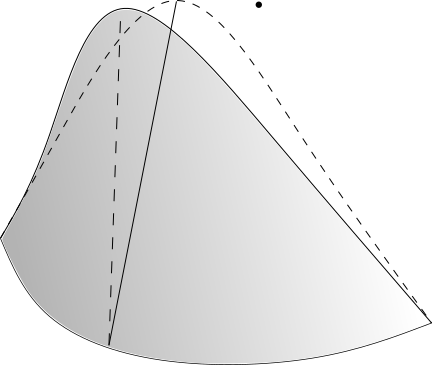
\includegraphics[width= 0.6\columnwidth]{./figure/Shifting.png}
				\caption{Shifting}
			\end{minipage}
			\begin{minipage}{0.4\hsize}
				\centering
				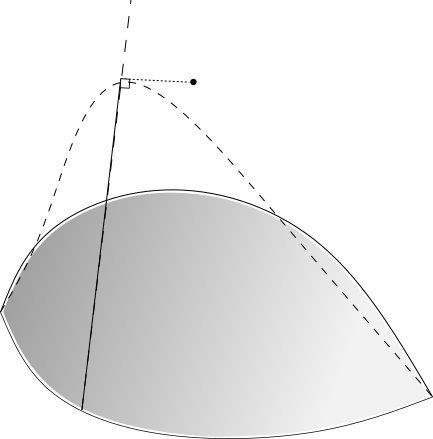
\includegraphics[width= 0.6\columnwidth]{./figure/Stretching.png}
				\caption{Stretching}
			\end{minipage}
		\end{figure}
		母線方向の曲線操作を行うStretchingについて説明する.この際,$ \varepsilon $に関する要求は以下にまとめられる.
		\begin{itemize}
			\item $ s=0,L $で$ \varepsilon(s) = 0 $
			\item $ \varepsilon \geq 0 \forall s \in [0,L]$
			\item $ \varepsilon'>0 \forall s \in [ 0,s_c ) $
			\item $ \varepsilon'<0 \forall s \in ( s_c ,L] $
			\item $ \varepsilon(s_c) = \varepsilon_p $(極大値制約)
		\end{itemize}
		3番目と4番目の式を自動的に解消するため,$ \varepsilon' $を常に定義域で$ 0 $より大きい保証がある$ f $を用いて以下のように記述できればよい.
		\begin{equation}\label{eq:ver_Sdot_eq}
			\varepsilon' = f(s)(s_c -s)%\sum_{i=1}^N a_i s^i 
		\end{equation}
		この$ f(s) $は,局所変形性に関する条件から,上記の制約下で以下を満たすように設計すればよい.
		\begin{equation}\label{eq:var_st_min}
			\min_{f} \int_{0}^L \varepsilon ds
		\end{equation}
		%$ \sum a_i s^i  >0\forall s \in [0,L]$が常に$ 0 $より大きければ,3番目と4番目の式を自動的に満たされるようになる.この文脈が常に成り立つ仮定で,局所的な変形が達成されるならば,以下の条件を満たす$ \bd{a} $を求める最適化問題になる.
		この問題は,Ritz法と同じ考えで,関数を基底関数の重み付き線形和で表現して係数に関する最適化問題に帰着させたいため,関数$ f $を以下のように記述する.
		\begin{equation}\label{eq:func_bd_a}
			f(s) = \sum_{i=1}^N a_i s^i 
		\end{equation}
		これを用いて目的関数を整理すれば目的関数は以下のように記述される.
		\begin{equation}\label{eq:objfunc_min}
			\min_{\bd{a}} \int_{0}^{L} \sum_{i=1}^N a_i \left(s_c \frac{s^{i+1}}{i+1} - \frac{s^{i+2}}{i+2} \right)= \sum_{i=1}^N a_i \left(s_c \frac{L^{i+2}}{(i+1)(i+2)} - \frac{L^{i+3}}{(i+2)(i+3)} \right)
		\end{equation}
		次に制約条件について考えると,$ \varepsilon(0)=0 ,\varepsilon(L)=0$が成り立つならば,2番目の制約は必ず満たされる.また,$ f(s)\geq 0 $の条件より
		\begin{equation}\label{eq:ineq_eq}
			\sum_{i=1}^N a_i s_j^i \geq 0 \;\; \forall s_j \in [0,L] 
		\end{equation}
		が成り立つ.今回は$ s $を離散化し不等式制約を代入した.また,制約条件は各々次式らで表される.
		\begin{equation}\label{eq:amend_cond_1}
			\sum_{i=1}^N a_i \left(s_c \frac{L^{i+1}}{i+1} - \frac{L^{i+2}}{i+2} \right) = 0
		\end{equation}
		\begin{equation}\label{eq:amend_cond_2}
			\sum_{i=1}^N a_i \left(\frac{s_c^{i+2}}{(i+1)(i+2)}\right) = \varepsilon_p
		\end{equation}
		このように,目的関数および制約条件は全て係数$ \bd{a} $について線形の形に書くことができるので,この最適化問題は$ \bd{a} $に関する線形計画問題として表現される.これを解けば,母線方向においては局所変形を達成することができる.
		
		この場合,母線方向については十分に議論することができるが,設計者が常に母線方向上に制御点を移動させるとは限らない.しかし,最大主曲率方向に移動させる場合には移動量が一意に決まるため,その移動によって点が改善するとは限らない.また,法線方向に移動させる際には,数値計算でしか解けない微分方程式を制約下で解く必要があり,計算コストが増大してしまう可能性がある.ある一定方向に一様に変形させる際には,微分方程式が解析的に解けることから,
		なんらかの方向で一様に曲面を変形させるShiftingという操作を行い,恣意的に母線方向を変更させると,Stretchingの動作を再び作用できると期待される.この行為では,なるべく変形を抑えながら点に近づく相反する2つの行為を同時に達成しなければならない.
		\begin{itemize}
			\item $ \int |\sum_{j=1}^{n} \varepsilon_j \bd{d}_j|^2 ds  $が最小であること
			\item $\min |\xv_{U,n}(s_c) + \varepsilon_{i+1} \bd{d}_{i+1} - \bd{C}| $
		\end{itemize}
		母線方向以外に変形させることから方向ベクトル$ \bd{d} $は,$ \bd{d} = \bd{d}_1(s_c) \cos \psi + \bd{\eta}(s_c) \sin \psi $と表すことが望ましい.$ \bd{d}_1(s_c),  \bd{\eta}(s_c) $は$ s=s_c $の時の方向を参照しているだけであり,ある一方向を表現していることに注意する.この時,上記で述べた2つの条件は次式のように表される.
		\begin{equation}\label{eq:No1_eq}
			\varepsilon_{c,i+1}^2 \int_{0}^{L} \exp \left[ \int_{s_c}^{s} 2\sigma_{i+1} (s) \right] + 2\varepsilon_{c,i+1} \bd{d}_{i+1} \cdot \left[\int_{0}^{L} \sum_{j=1}^{i} \varepsilon_j \bd{d}_j \exp \left[ \int_{s_c}^{s} 2\sigma_{i+1} (s) \right] \right] + \int_{0}^{L} |\sum_{j=1}^{i} \varepsilon_j \bd{d}_j|^2 ds
		\end{equation}
		\begin{equation}\label{eq:No2_eq}
			\varepsilon_{c}^2 -2 \varepsilon_{c} \bd{d}\cdot (\bd{C}-\xv_{U,n}) + |\bd{C}-\xv_{U,n}|^2
		\end{equation}
		式(\ref{eq:No2_eq})が最小値をとる条件は,以下のように表される.
		\begin{equation}\label{eq:var_eq_with_psi}
			\varepsilon_{c} = \bd{d}_1 \cdot (\bd{C} - \xv_{U,n}) \cos \psi + \etav \cdot (\bd{C}-\xv_{U,n}) \sin \psi
		\end{equation}
		これを式(\ref{eq:No1_eq})とを連立することで,$ \psi $の式として表すことができ,最小化する条件を達成することで,$ \psi $を求めることができる.(計算略)
		この動作を,誤差が$ \delta $以下になるまで反復させることで,曲面の局所変形を達成できると考えられる.
    	
    \section{結果}
    この数値実験では,2つの円弧の間に形成された曲面を$ s=0.2 $の時の点を,$\bd{C} = [ 0.241197 0.308751 0.480096 ]$に変更したい場合を想定した結果となる.
    	\begin{figure}[H]
    		\begin{minipage}{0.5\hsize}
    			\centering
    			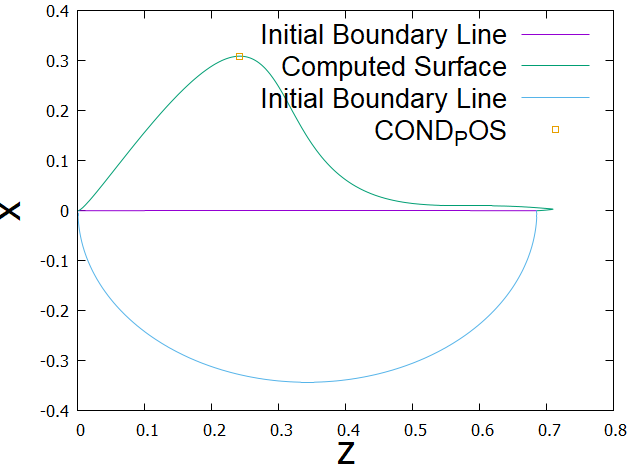
\includegraphics[width = 1.0\columnwidth]{figure/0409/ObtainedRidgeLinefromz-x.png}
    			\caption{z-x plane }
    		\end{minipage}
	    	\begin{minipage}{0.5\hsize}
	    		\centering
	    		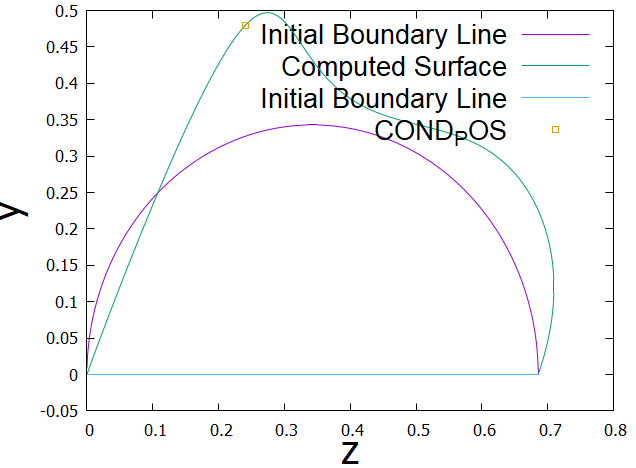
\includegraphics[width = 1.0\columnwidth]{figure/0409/ObtainedRidgeLinefromz-y.png}
	    		\caption{z-y plane }
	    	\end{minipage}
    	\end{figure}
   	\begin{figure}[H]
    		\centering
    		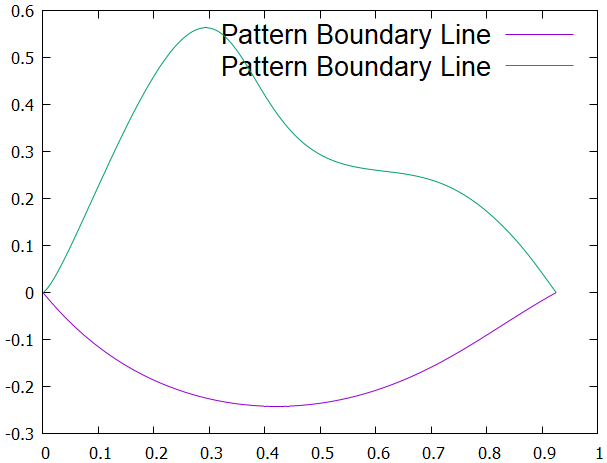
\includegraphics[width = 0.4\columnwidth]{figure/0409/Patt2.png}
    		\caption{z-y plane }
    \end{figure}
	この結果より,非常に曲線および曲面を局所的に変更することができたことが読み取れる.
		
	\section{次回のMTGについて(終了後記載)}
	\begin{itemize}
		\item  
		\item 
	\end{itemize}
	###
	\newpage
%\vspace{10cm}
%%%%%%%%%%%%%%%%%%%%%%%%%%%%%%%%%%%%%%
% 3.達成できなかったこととその問題点
	%\articleSPRthree
	
%%%%%%%%%%%%%%%%%%%%%%%%%%%%%%%%%%%%%%

%\vspace{14cm}
%%%%%%%%%%%%%%%%%%%%%%%%%%%%%%%%%%%%%%
	%\articleSPRfour
	%\articleSPRfive
\end{document}
